\documentclass[11pt, a4paper]{article}
%\usepackage{proj1}
\usepackage{natbib}
\usepackage{fancyhdr}  
\usepackage{subcaption}
\usepackage{caption}
\usepackage{graphicx}
\usepackage{numprint}
\usepackage{multirow}
\linespread{1.25} 
\setlength{\parindent}{0cm}
\graphicspath{{Images/}}
\usepackage{hyperref}
\usepackage{amsmath}
\usepackage{amsfonts}
\usepackage{amssymb}
\usepackage{amsthm}
\usepackage{mathtools}
\usepackage{commath}
\usepackage{bbm}

%\usepackage[sc,osf]{mathpazo}
\usepackage{subcaption}
\usepackage[a4paper, top=1in, left=1.0in, right=1.0in, bottom=1in, includehead, includefoot]{geometry} %Usually have top as 1in

\usepackage{listings}
\usepackage{color} %red, green, blue, yellow, cyan, magenta, black, white
\definecolor{mygreen}{RGB}{28,172,0} % color values Red, Green, Blue
\definecolor{mylilas}{RGB}{170,55,241}


\hypersetup{colorlinks,linkcolor={black},citecolor={blue},urlcolor={black}}
\usepackage{color}
\urlstyle{same}


\theoremstyle{definition}
\newtheorem{definition}{Definition}[section]

\newcommand{\adja}{q_a}
\newcommand{\adjb}{q_b}
\newcommand{\adjaB}{q_{a,\partial \Omega}}
\newcommand{\adjbB}{q_{b,\partial \Omega}}
\newcommand{\adjB}{q_{\partial \Omega}}
\newcommand{\Adja}{\mathbf{p}}
\newcommand{\Adjb}{q}
\newcommand{\adj}{q}
\newcommand{\Adjc}{{q}_{\partial \Omega}}
\newcommand{\ra}{\rho_a}
\newcommand{\rb}{\rho_b}
\newcommand{\w}{\mathbf{w}}
\newcommand{\f}{\mathbf{f}}
\newcommand{\ve}{\mathbf{v}}
\newcommand{\n}{\mathbf{n}}
\newcommand{\h}{\mathbf{h}}
\newcommand{\K}{\mathbf{K}}
\newcommand{\hr}{\widehat \rho}
\newcommand{\jf}{\mathbf j}

%	\begin{figure}[h]
%		\centering
%		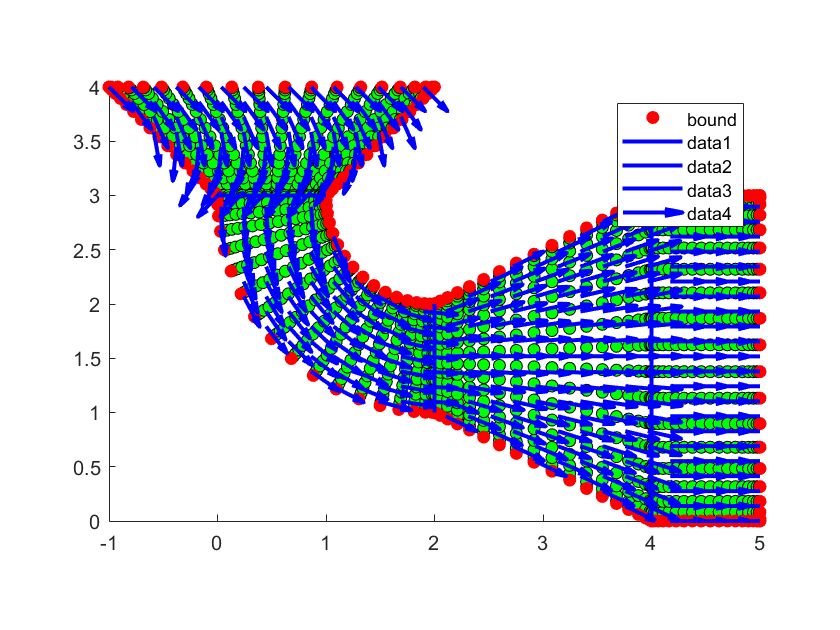
\includegraphics[scale=0.35]{F1.png}
%		\caption{Forward $\rho$ for $a = 0.01$} 
%		\label{F1}
%	\end{figure}

\begin{document}


\section{Issue with periodic interpolation}
	Define a function on a PeriodicBox as:
	\begin{align*}
		f = \exp(-5(y_1 - 1.5)^2 - 5(y_2 - 0.7)^2),
	\end{align*}	
	and choose the domain $[0,2]\times [0,1]$.
	Then I choose a number of points for my domain, $N$ and a number of plotting points $N_p$. We can see in Figure \ref{F1}, that if $N_p \neq N$, we have an interpolation issue in the periodic direction (top/bottom).
		\begin{figure}[h]
		\centering
		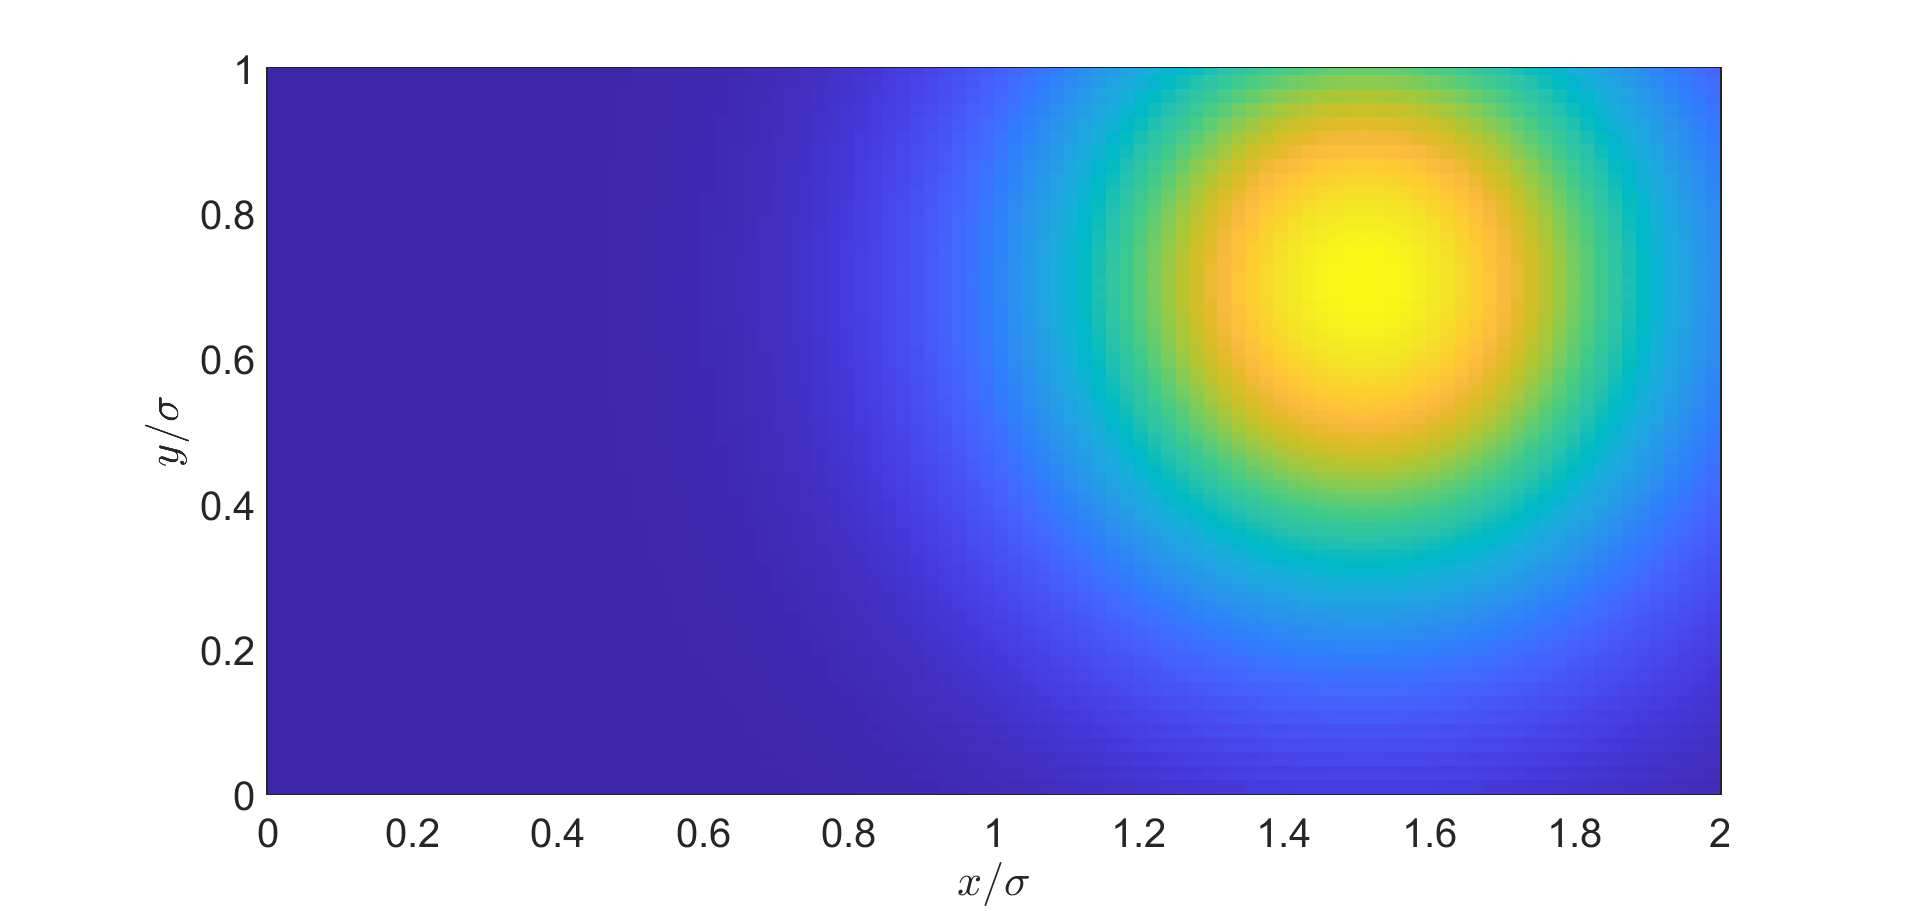
\includegraphics[scale=0.15]{N100a.png}
		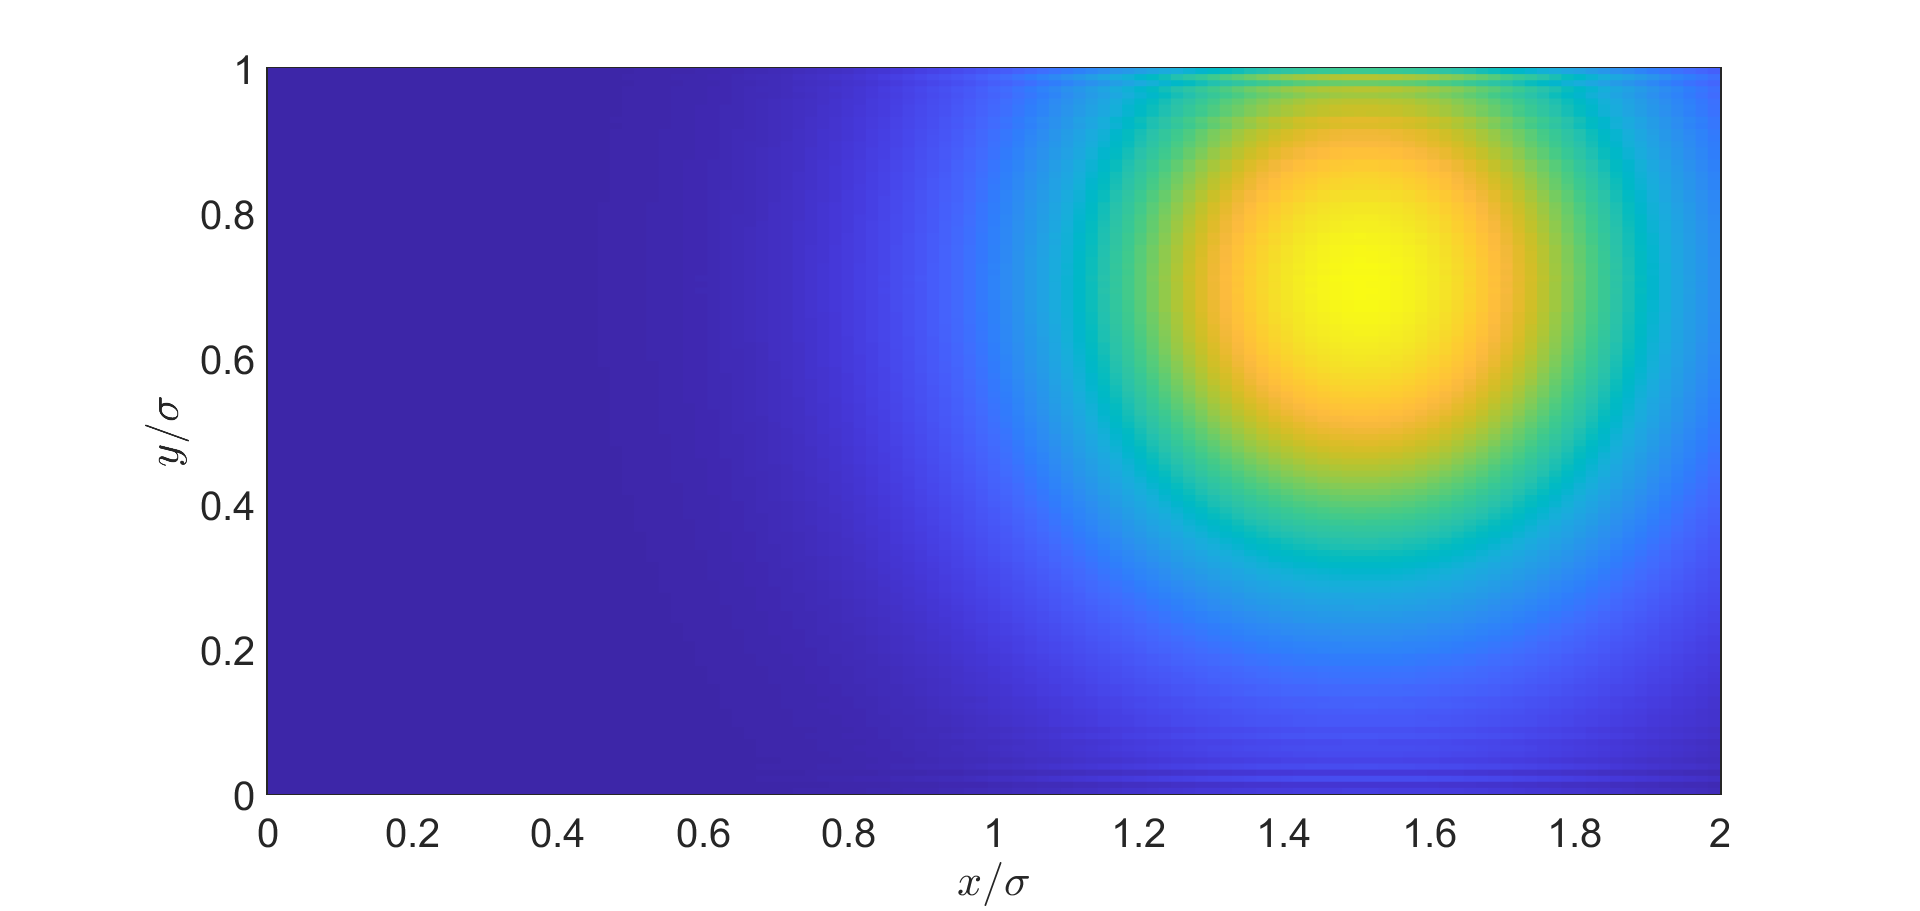
\includegraphics[scale=0.15]{N100b.png}
		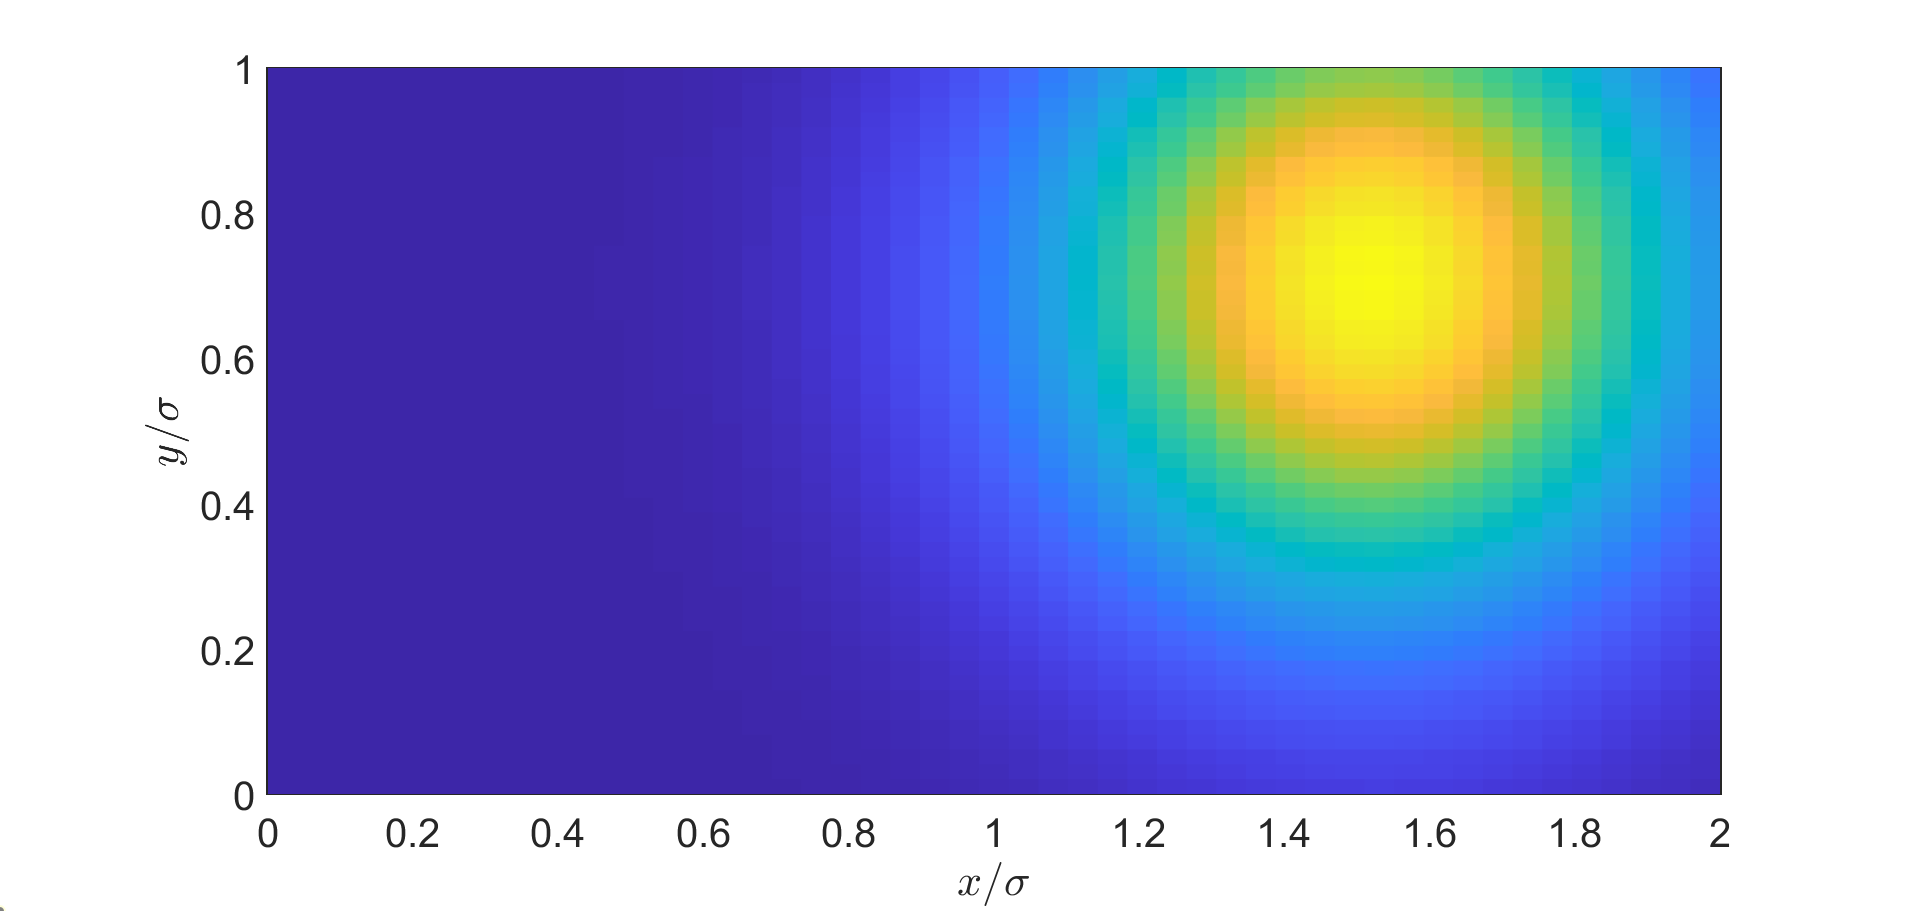
\includegraphics[scale=0.15]{N50a.png}
		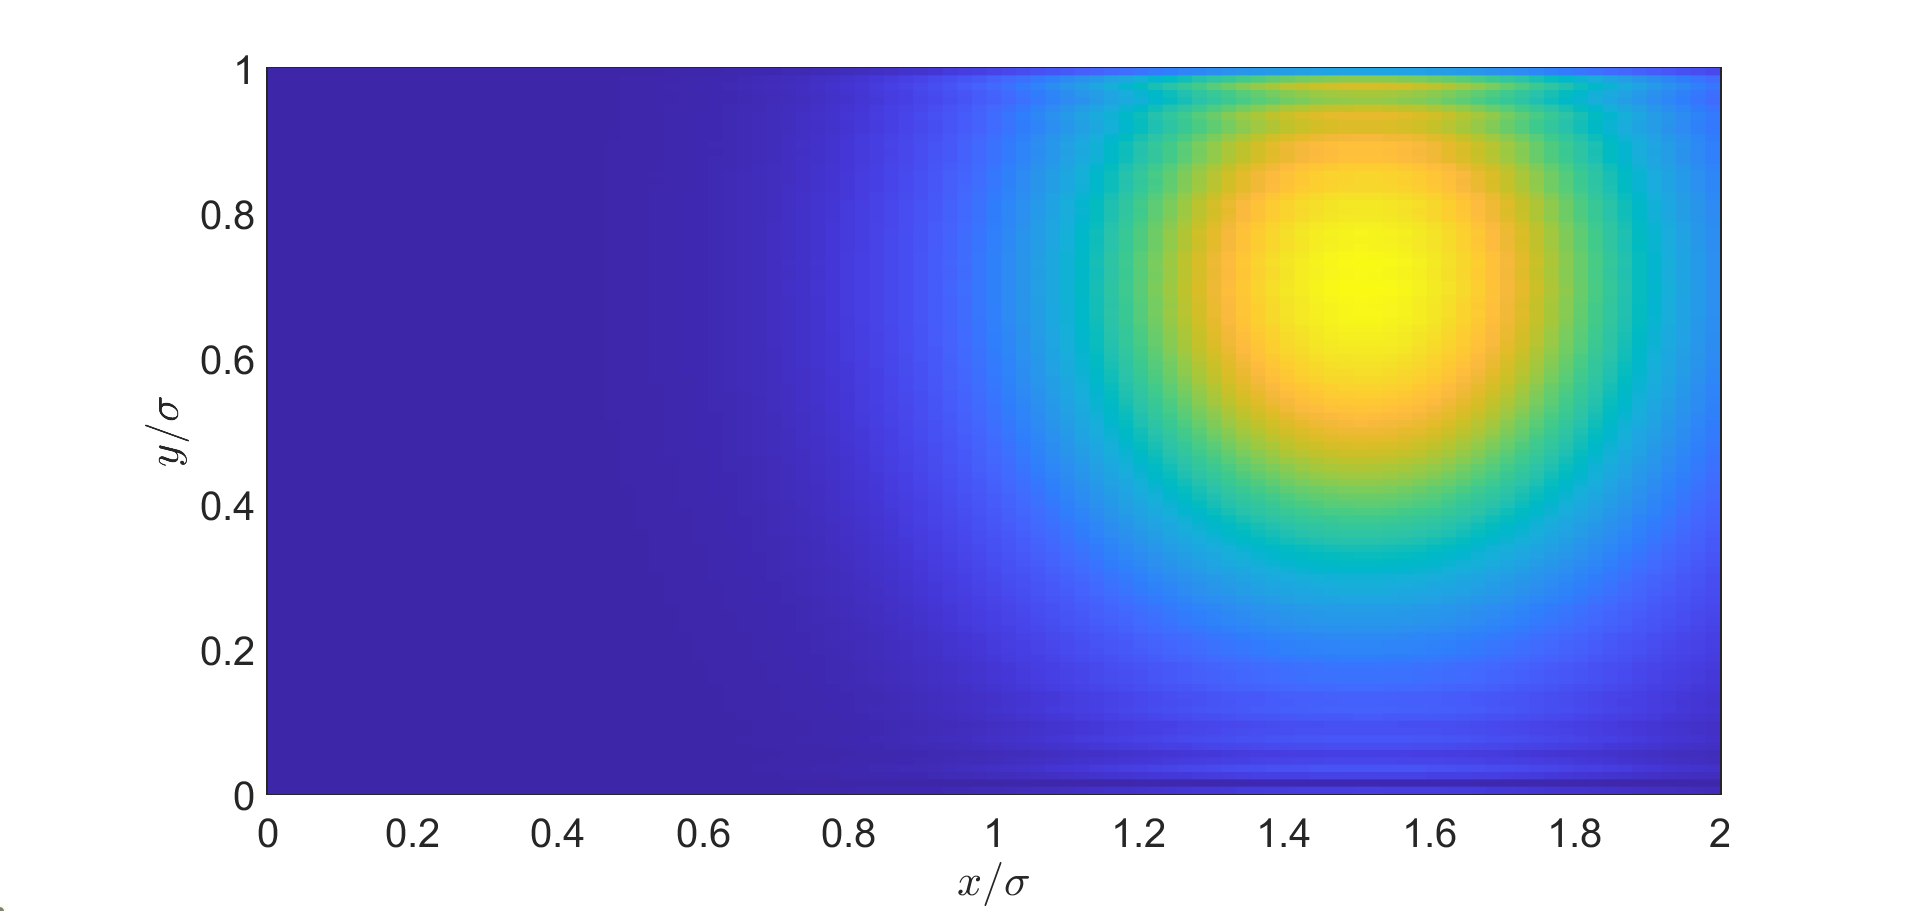
\includegraphics[scale=0.15]{N50b.png}
		\caption{Top left: $N = N_p = 100$, top right: $N = 100,\ \ N_p = 120$, bottom left: $N = N_p = 50$, bottom right: $N = 50,\ \ N_p = 100$.} 
		\label{F1}
	\end{figure}
	When trying to interpolate the Box forward problem onto the PeriodicBox grid, there is another problem, even when choosing $N = N_p$. 
	For $N = N_p = 50$, we get the results displayed in Figure \ref{F2}. If we choose $N_p = 100$ we can see the additional issue of interpolation error, as demonstrated in Figure \ref{F1}, see Figure \ref{F3}.
	\begin{figure}[h]
		\centering
		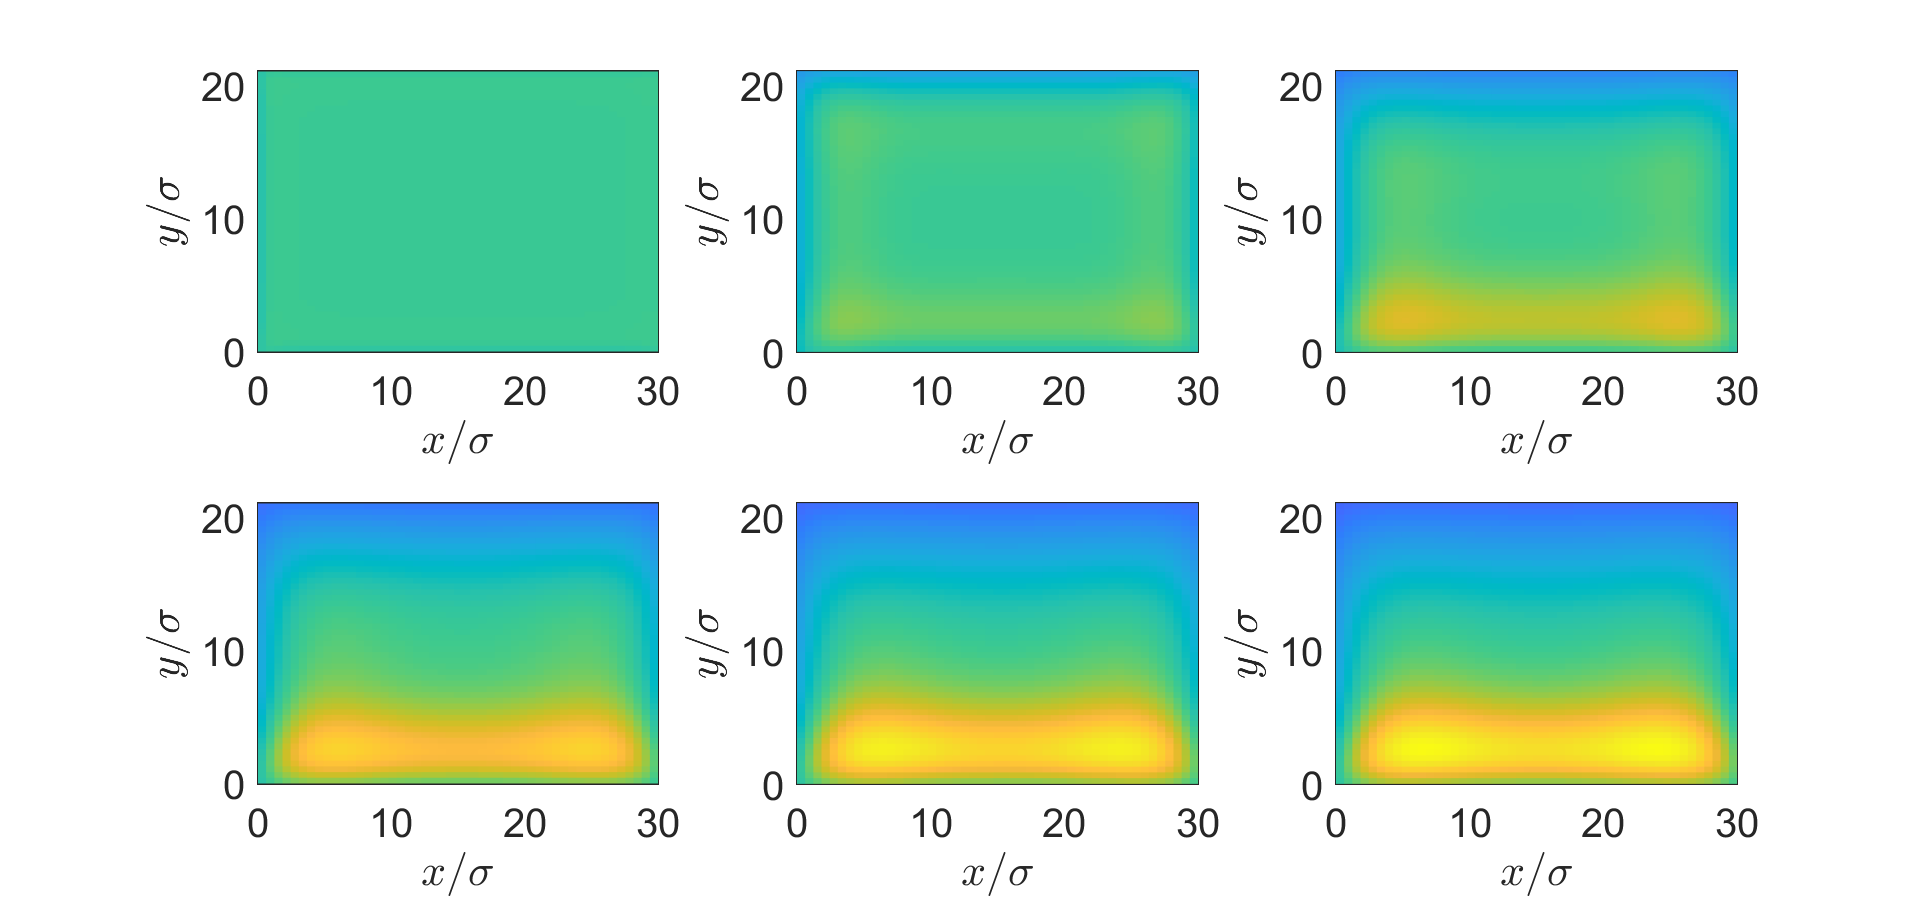
\includegraphics[scale=0.3]{Original.png}
		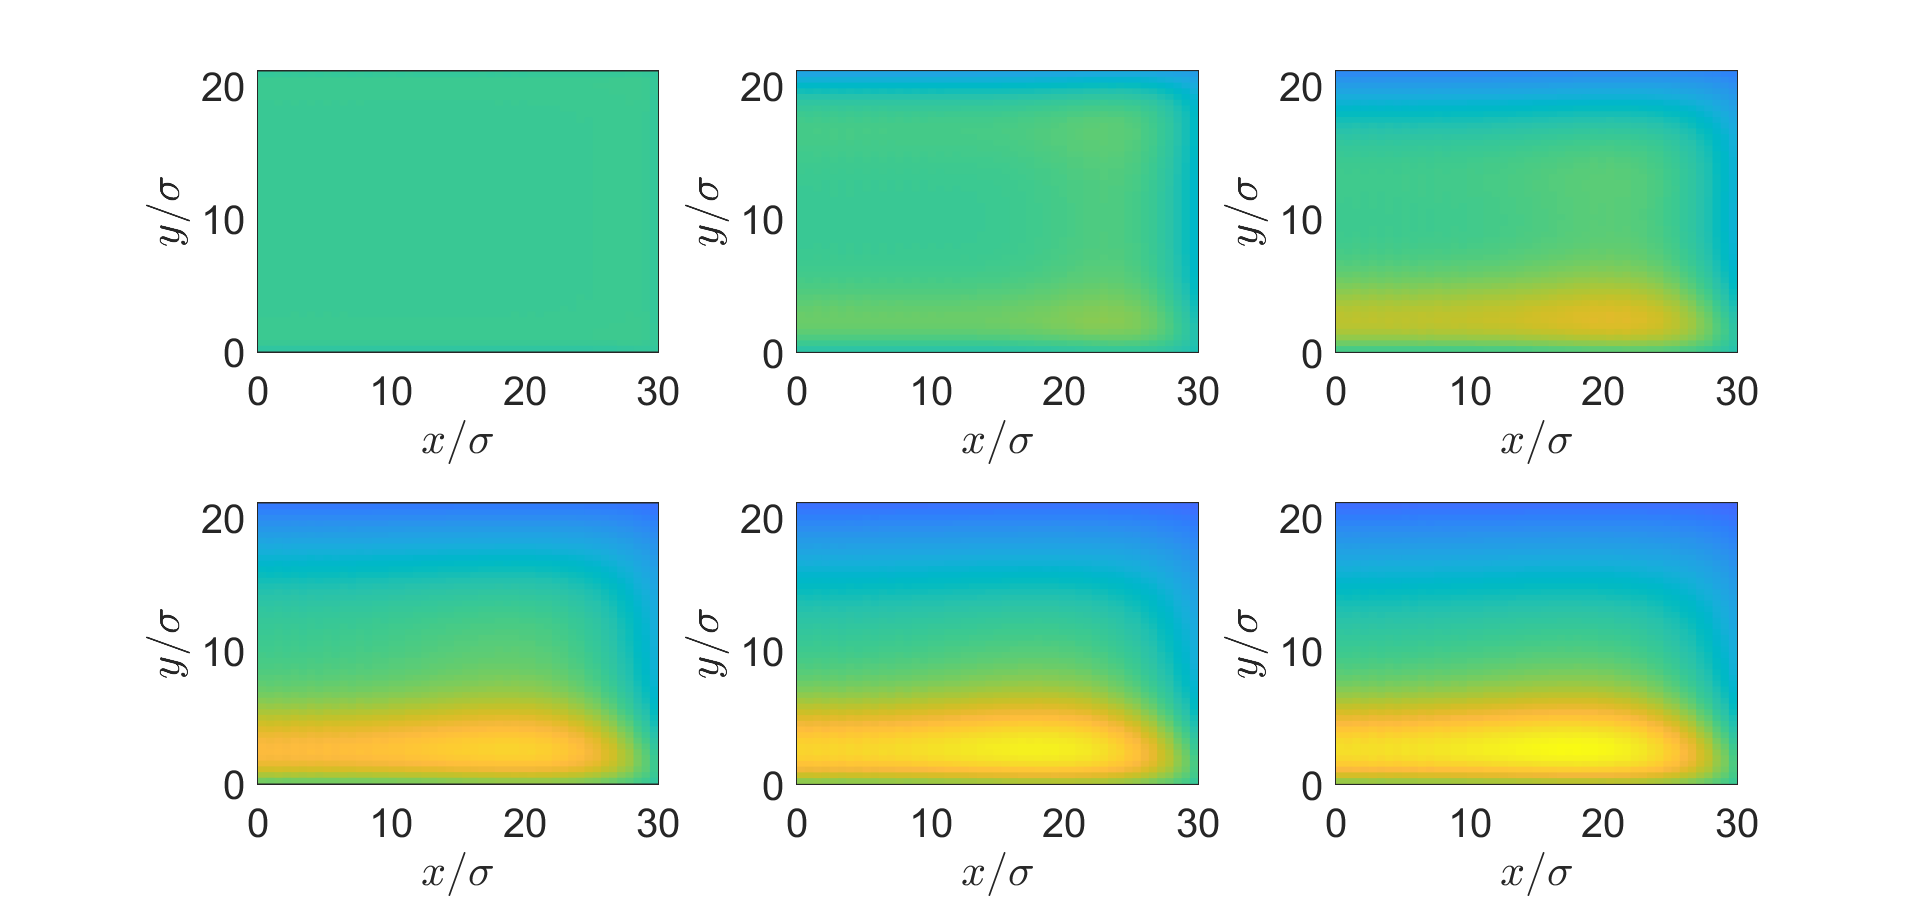
\includegraphics[scale=0.3]{Periodic.png}
		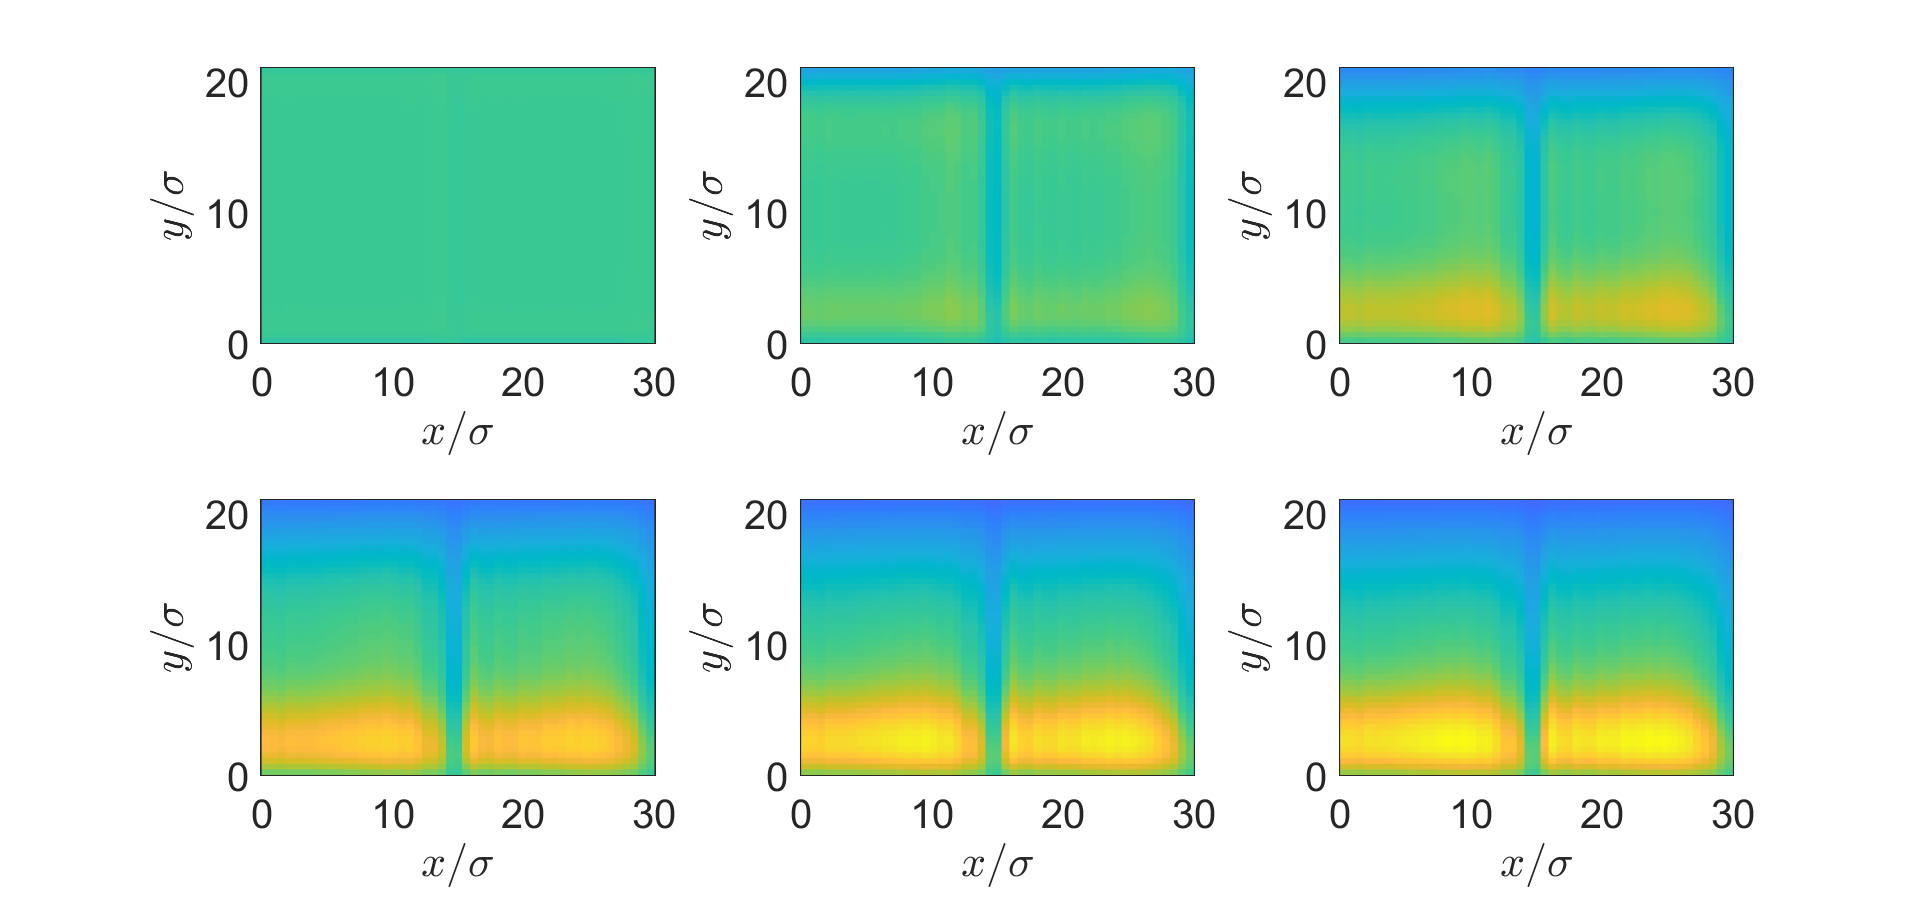
\includegraphics[scale=0.3]{Interpolated.png}
		\caption{Original result, interpolated onto periodic grid, interpolated back on box grid, $N_p = N = 50$} 
		\label{F2}
	\end{figure}
	\begin{figure}[h]
		\centering
		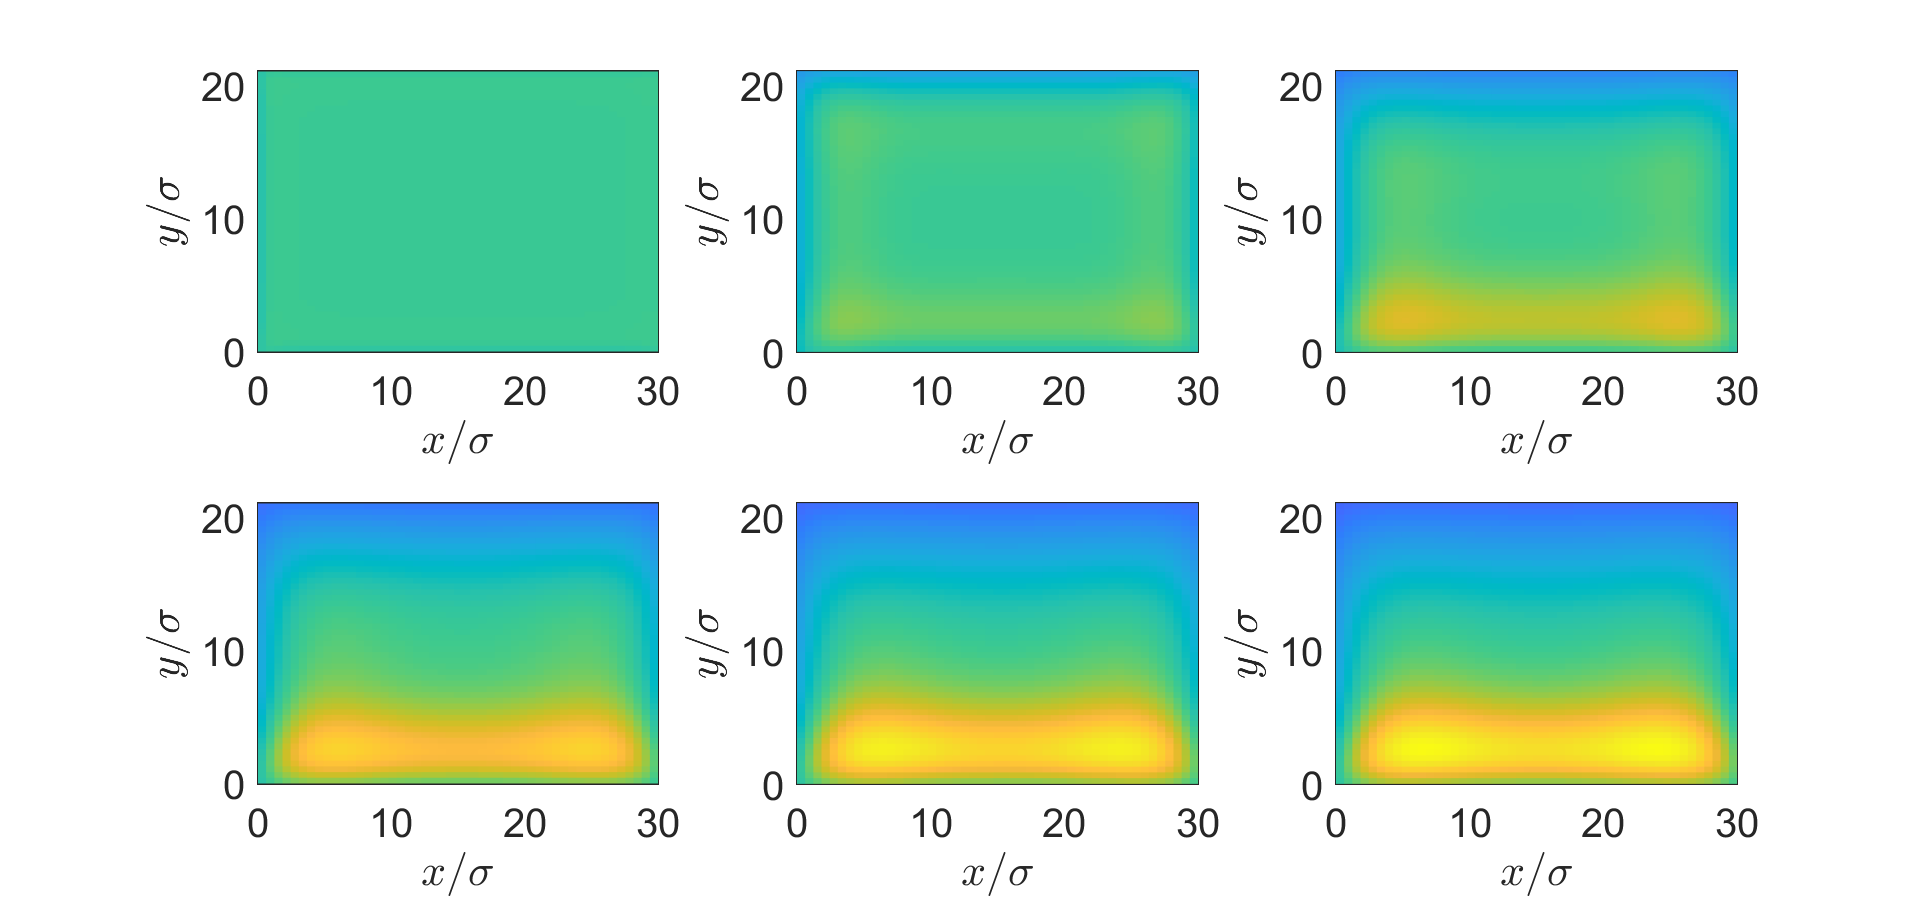
\includegraphics[scale=0.3]{Original.png}
		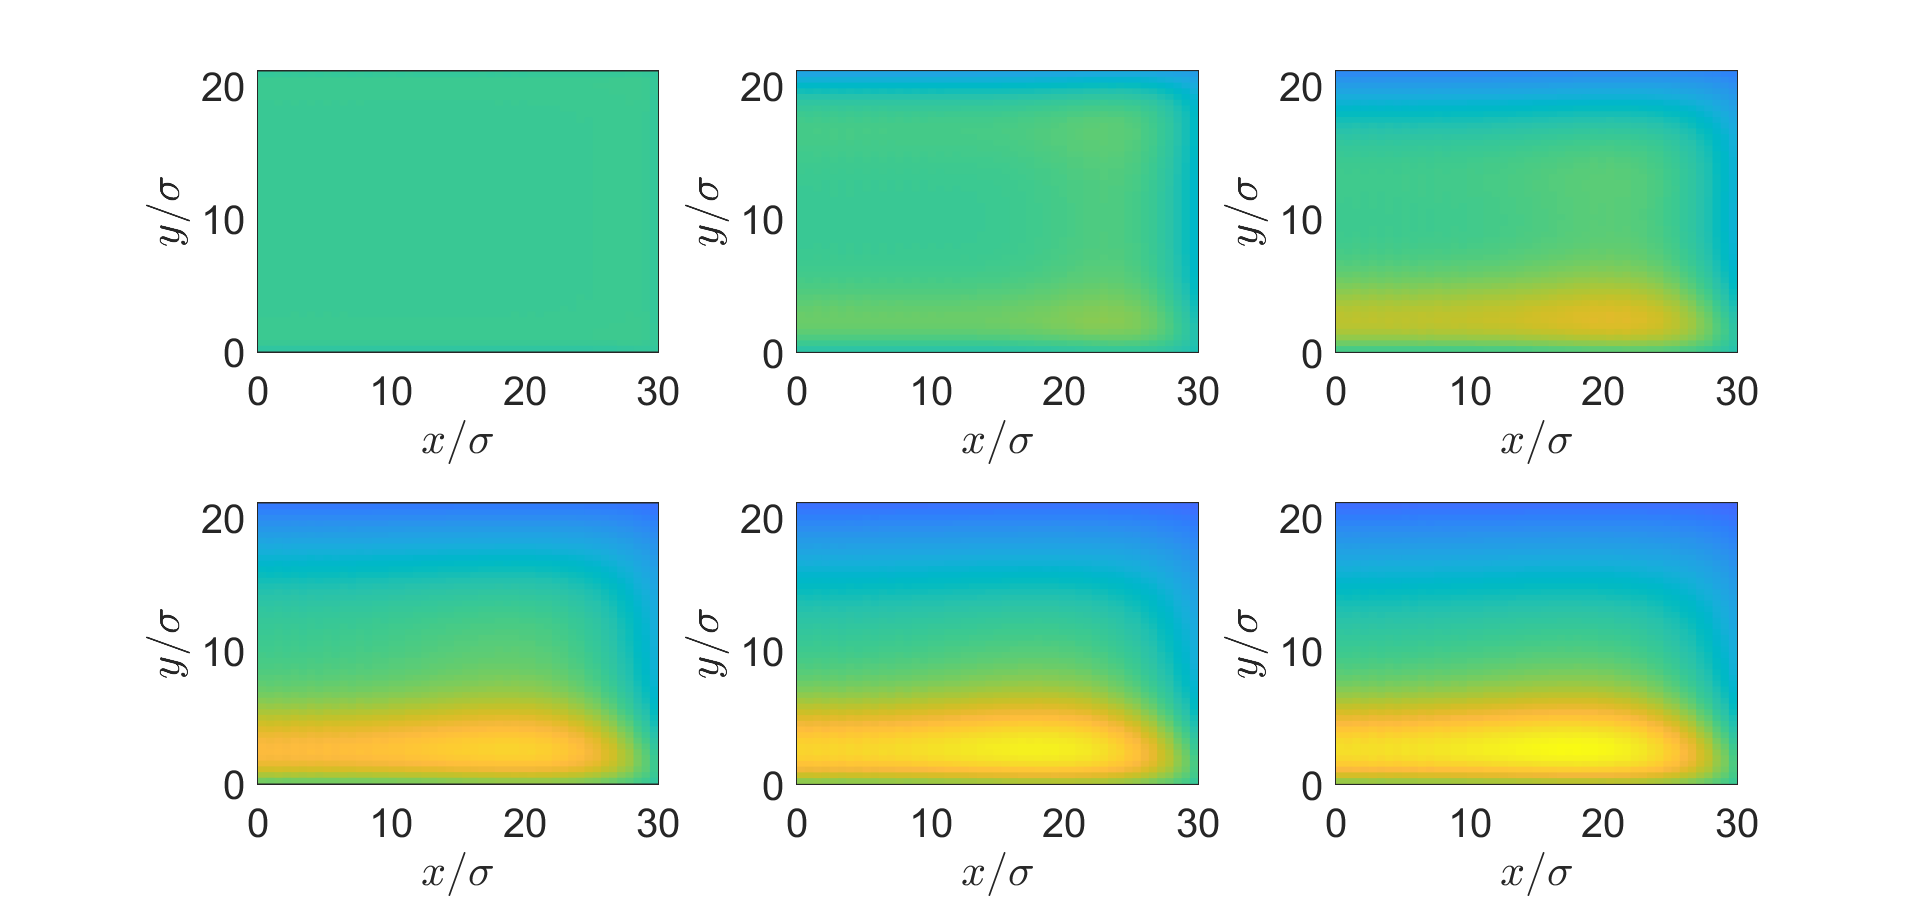
\includegraphics[scale=0.3]{Periodic.png}
		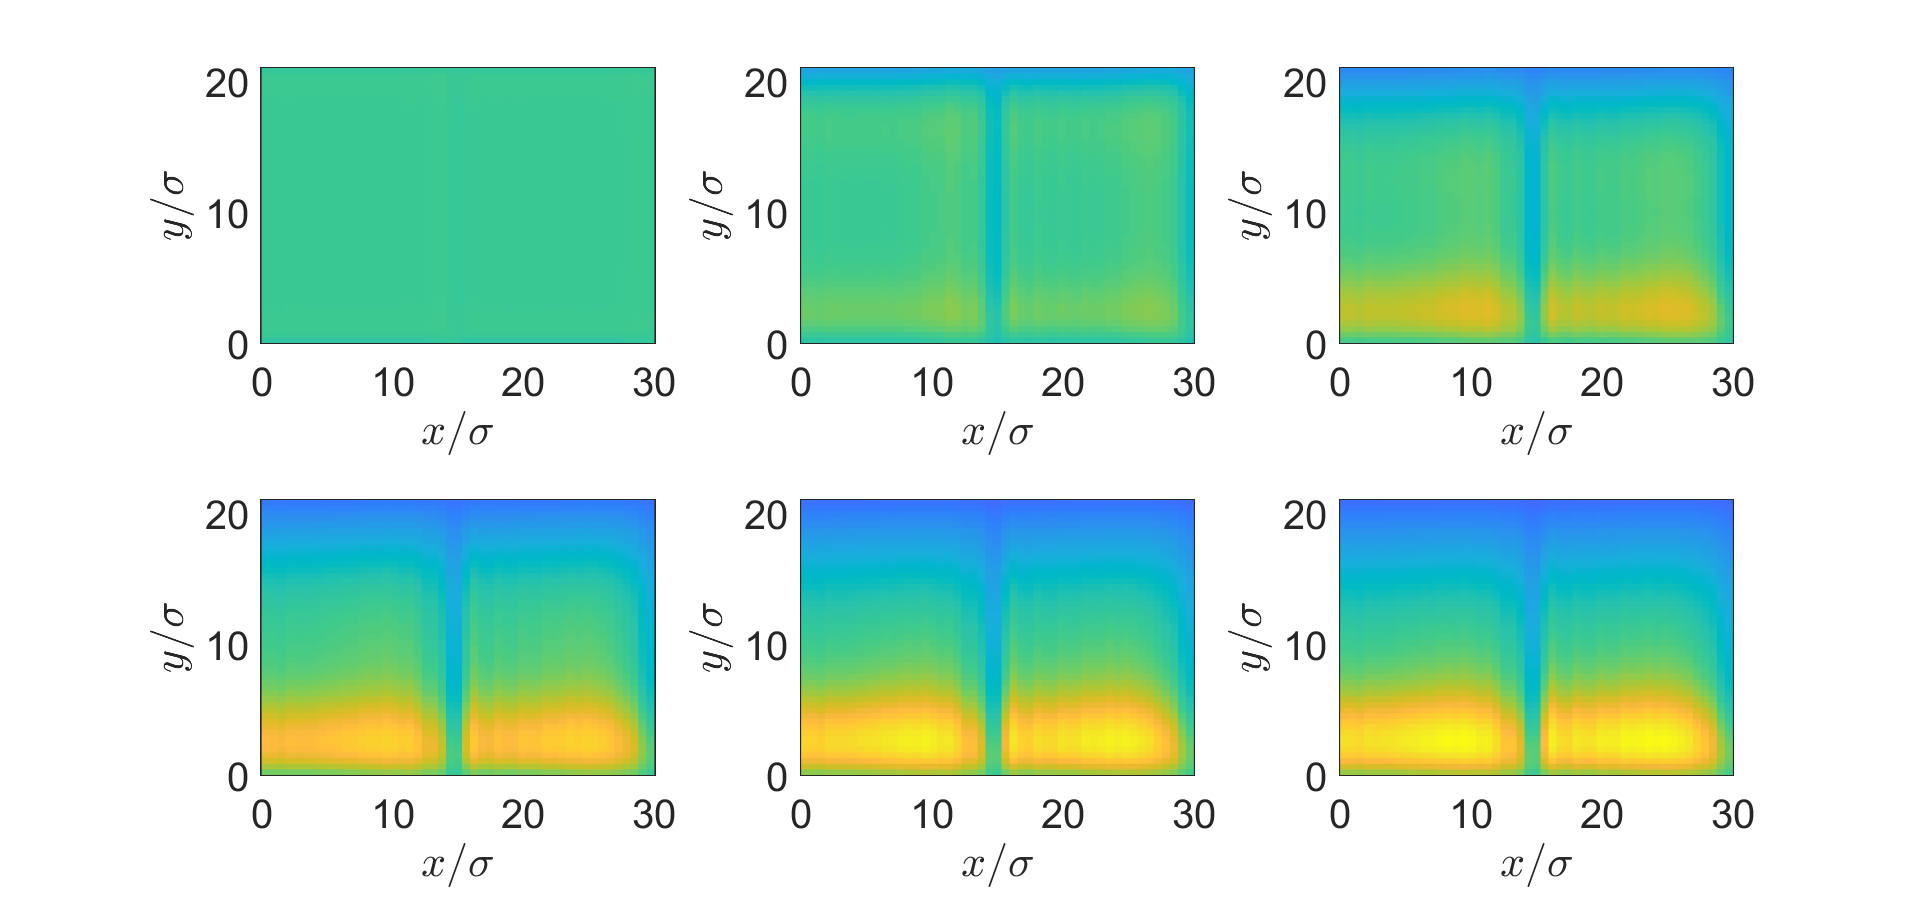
\includegraphics[scale=0.3]{Interpolated.png}
		\caption{Original result, interpolated onto periodic grid, interpolated back on box grid, $N = 50$, $N_p = 100$} 
		\label{F3}
	\end{figure}
		
		
\section{Periodic OCP}
We choose $\hr$ to be the forward problem in a box with the typical sedimentation setup. We choose $N = 20$, $n = 30$. We then give this to the optimal control problem in a periodic box. Without interpolating on the new grid, the box forward problem gets squashed into the middle a little, compare Figure \ref{F2} and Figure \ref{F4}.
We then get that $J_{FW} = 0.4351$ and $J_{Opt} = 0.1032$. As expected, the control forces the particles inward. Interestingly, it also pushes them upward, which makes sense when comparing to the periodic forward problem. Results are displayed in Figure \ref{F4}.
	\begin{figure}[h]
		\centering
		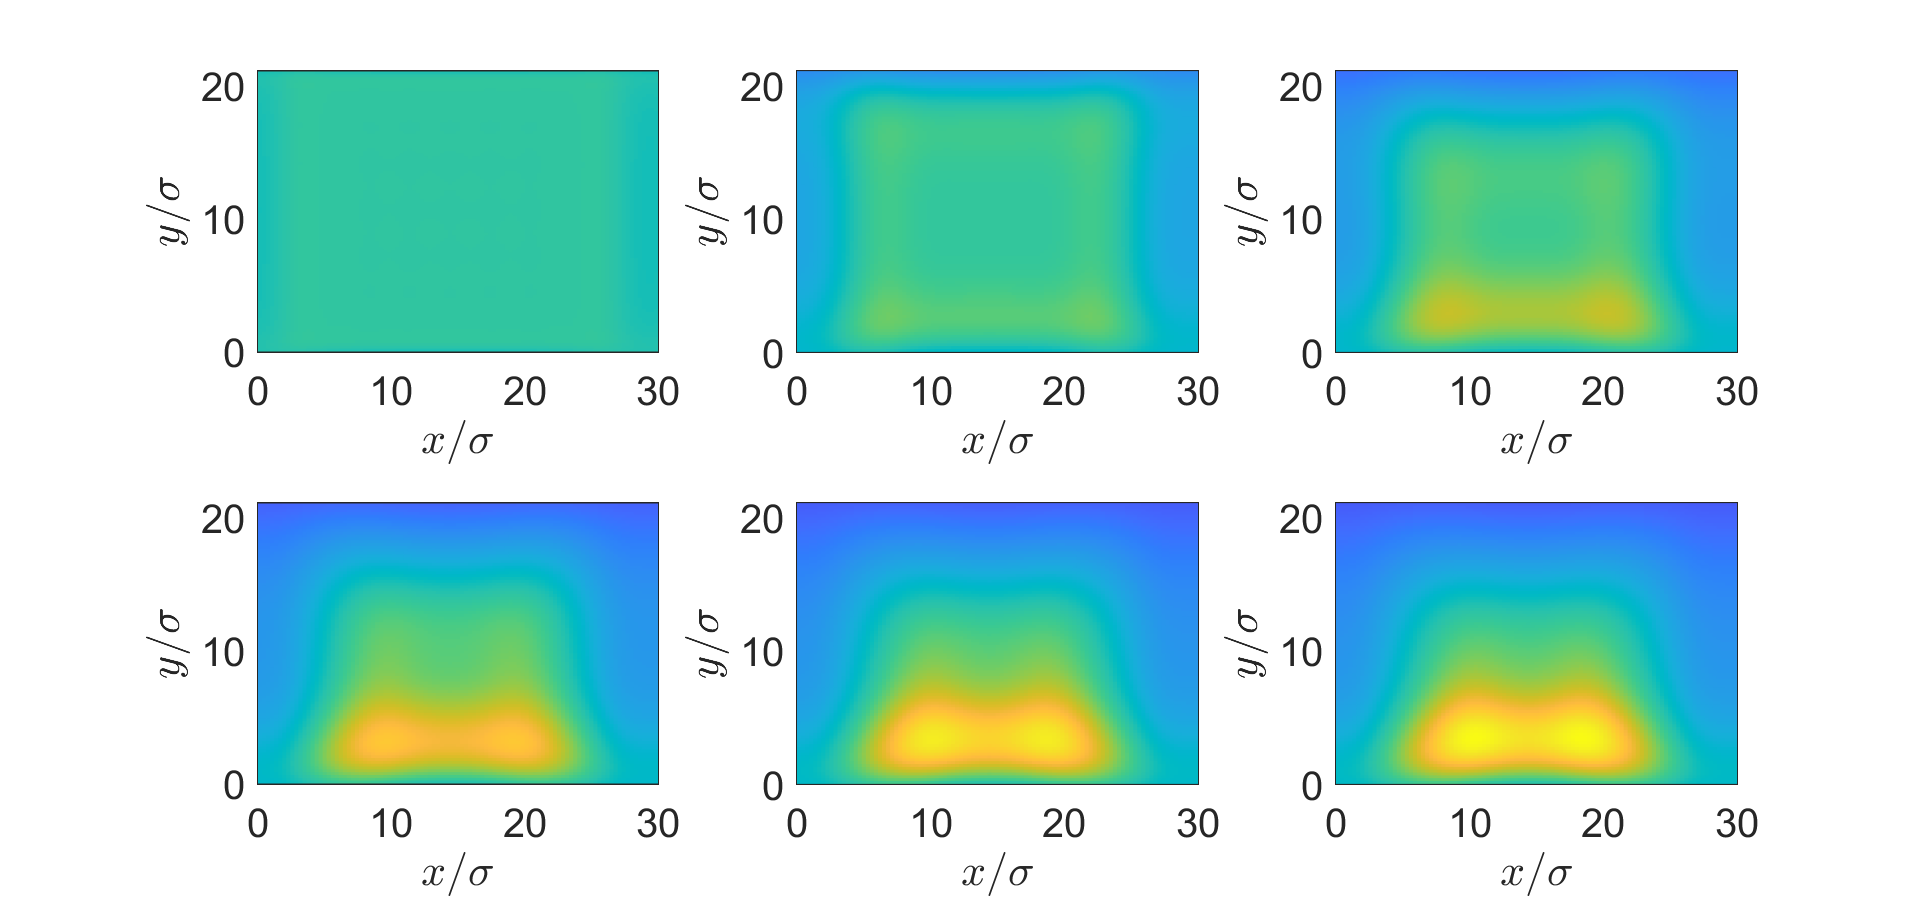
\includegraphics[scale=0.3]{rhoTarget.png}
		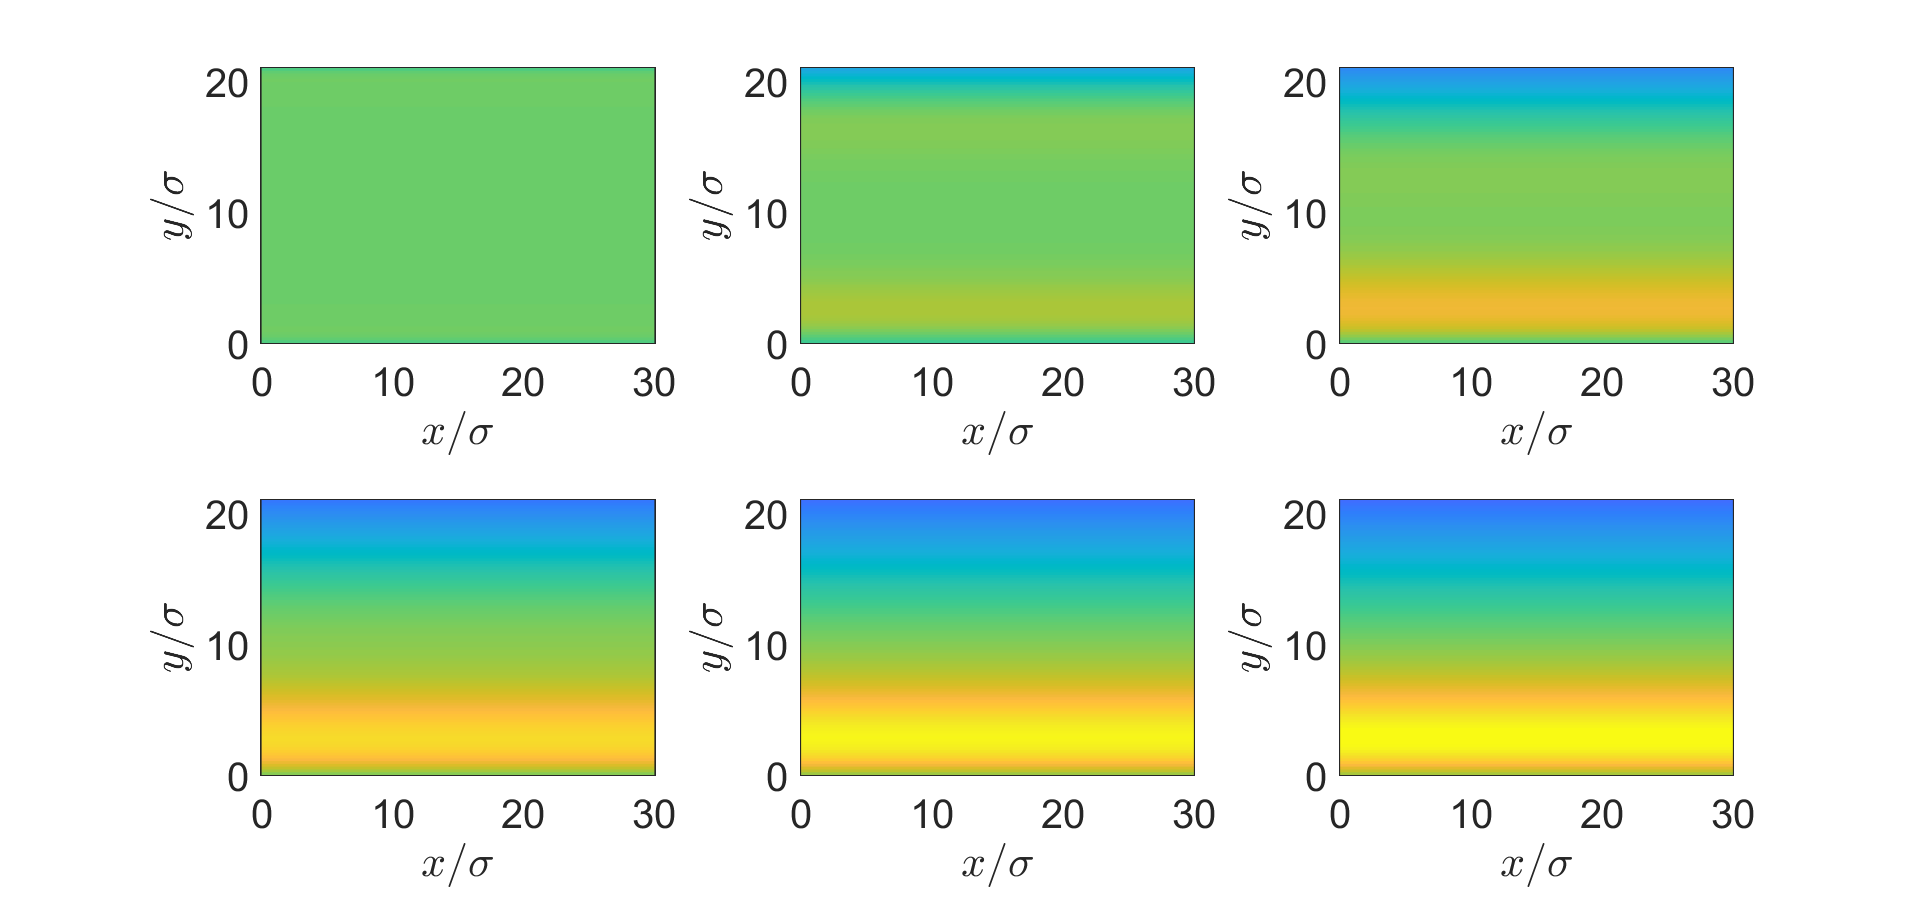
\includegraphics[scale=0.3]{rhoFWPeriodic.png}
		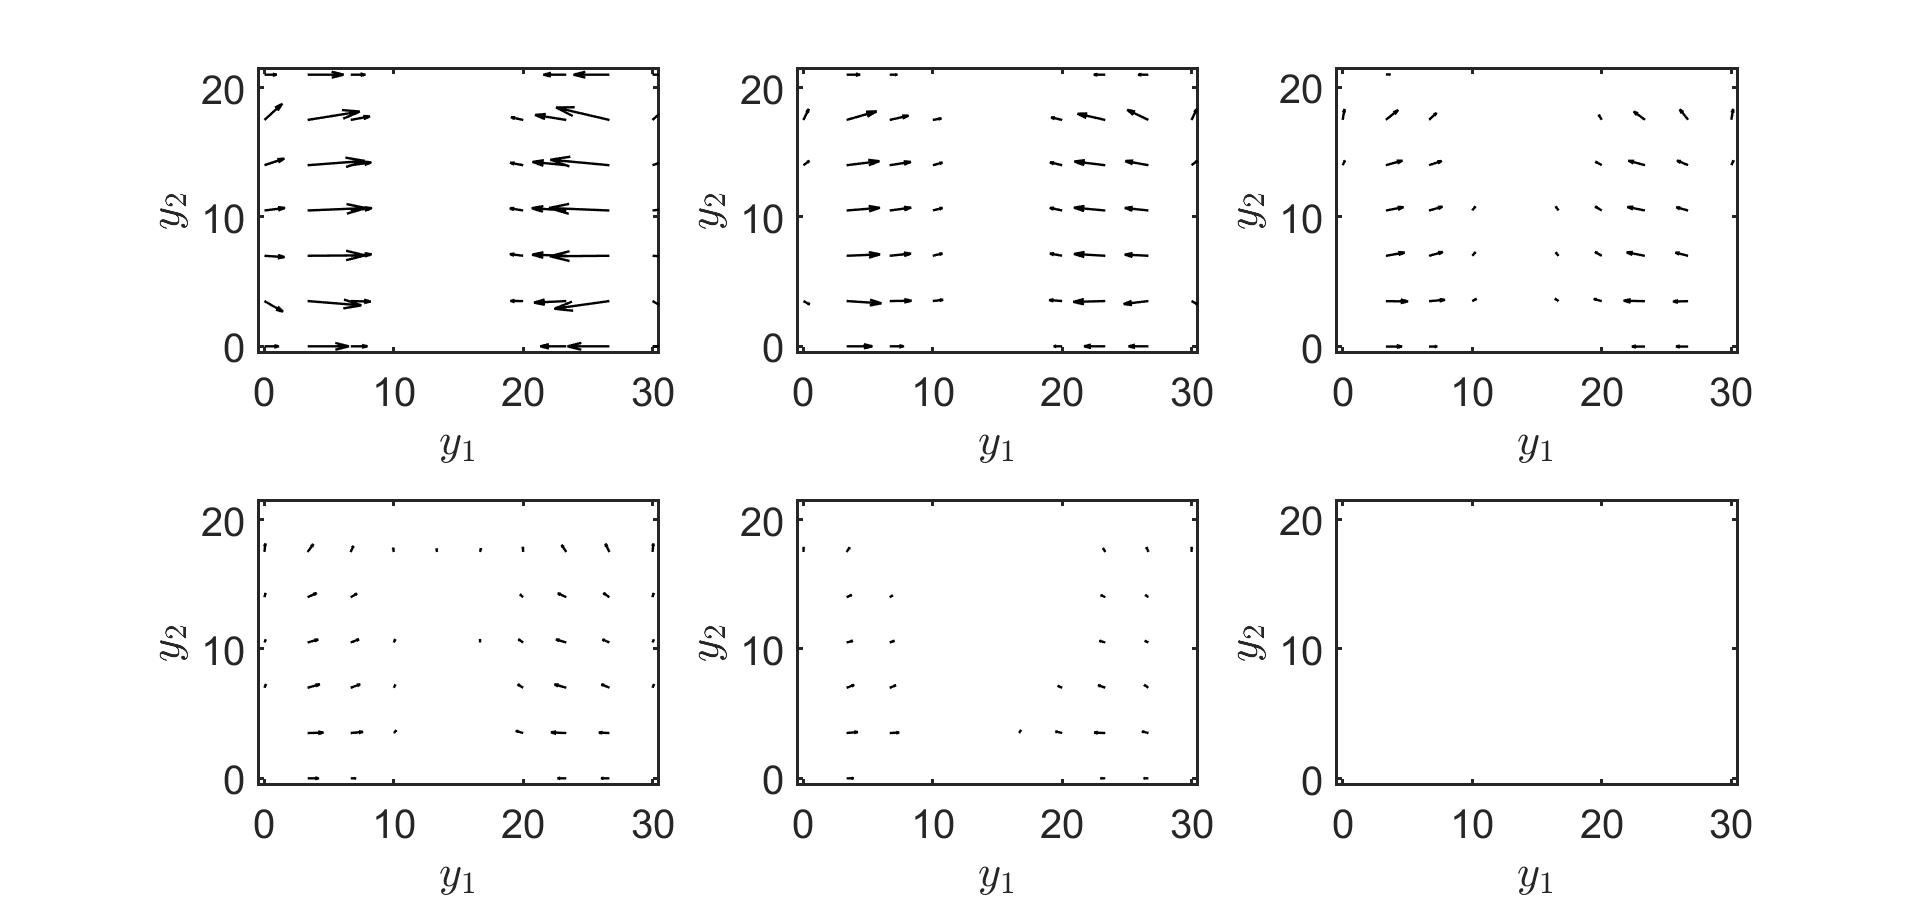
\includegraphics[scale=0.3]{Control.png}
		\caption{$\hr$, forward $\rho$ and optimal control} 
		\label{F4}
	\end{figure}

\section{Periodic Boundary Conditions for a General Flux}

We consider the advection diffusion equation with periodic boundary conditions and a corresponding OCP:
\begin{align*}
	&\min \frac{1}{2}|| \rho - \hr||^2 + \frac{\beta}{2}||\w||^2\\
	&\text{subject to:}\\
	&\frac{\partial \rho}{\partial t} = \nabla \cdot \left(\nabla \rho - \rho \w\right) = -\nabla \cdot \jf\\
	& \rho|_{\partial \Omega_l} = \rho|_{\partial \Omega_r}\\
	& \rho|_{\partial \Omega_t} = \rho|_{\partial \Omega_b}\\
	& - \jf \cdot \n |_{\partial \Omega_l}= - \jf \cdot \n|_{\partial \Omega_r}
\end{align*}
such that $\partial\Omega_l \cup \partial\Omega_r = \partial \Omega$ and the abbreviations corresponding to left and right respectively. Top and bottom boundaries are omitted, since, as shown in the previous section, they follow analogously and are independent of the results on the left and right boundary.
The relevant part of the Lagrangian is then:
\begin{align*}
	\mathcal{L} &= ... -\int_0^T \int_\Omega \left(\frac{\partial \rho}{\partial t} + \nabla \cdot \jf\right)q dr dt - \int_0^T \int_{\partial \Omega_l} \left(- \rho q_1 - \jf \cdot \n q_2 \right) dr  + \int_{\partial \Omega_r} \left(\rho q_1 +  \jf \cdot \n q_2  \right)  dr .
\end{align*}
Integrating by parts, and omitting terms in $\Omega$, gives:
\begin{align*}
	\mathcal{L} &= ... - \int_0^T \int_{\partial \Omega} q \jf  \cdot \n + \mathbf{k}(\rho, q) \cdot \n  dr dt - \int_0^T \int_{\partial \Omega_l} \left(- \rho q_1 - \jf \cdot \n q_2 \right)   dr  + \int_{\partial \Omega_r} \left(\rho q_1 + \jf \cdot \n q_2 \right)   dr, 
\end{align*}
where $\mathbf{k}$ are any terms arising from integrating by parts a second time.
We now need to take the Frech\'et derivative of $\jf$ with respect to $\rho$. This cannot be done in general, because $\jf$ does not only depend on $\rho$ but also on $\mathbf r$. In each case we need to calculate:
\begin{align*}
	\jf'(h) := \jf (\rho + h) - \jf (\rho).
\end{align*}
Similarly, we need to take the derivative of $\mathbf k$ and denote it by $\mathbf{k}'$.
Denoting this Frech\'et derivative by $\jf'(h)$ we can write out further terms as follows:
\begin{align*}
	\mathcal{L}_\rho &= ... - \int_0^T \int_{\partial \Omega} q \jf'(h)   \cdot \n + \mathbf{k}' \cdot \n dr dt - \int_0^T \int_{\partial \Omega_l} \left(- h q_1 - \jf'(h)  \cdot \n q_2 \right)   dr  + \int_{\partial \Omega_r} \left(h q_1 + \jf'(h)  \cdot \n q_2 \right)   dr dt. 
\end{align*}
When writing out the terms explicitly we pay attention to the fact that $\n|_{\partial \Omega_l} = - \n|_{\partial \Omega_r}$ and $\n|_{\partial \Omega_t} = - \n|_{\partial \Omega_b}$.
\begin{align*}
	\mathcal{L}_\rho &= ... - \int_0^T \int_{\partial \Omega_l} \left(- h q_1 + q \jf'(h)   \cdot \n  + \mathbf{k}' \cdot \n- \jf'(h)  \cdot \n q_2 \right)   dr  \\
	&+ \int_{\partial \Omega_r} \left(h q_1 - q \jf'(h)   \cdot \n - \mathbf{k}' \cdot \n+ \jf'(h)  \cdot \n q_2 \right)   dr dt .
\end{align*}
In order to proceed further, we need to split up $\jf'(h)$ into two parts as follows:
\begin{align*}
	\jf'(h) = \jf'_1(h) + h \jf'_2,
\end{align*}
so that $\jf'_1$ is applied to $h$, since it depends on $\mathbf{r}$ as well (e.g. the Frech\'et derivative of $\nabla \rho$) and $\jf'_2$ is applied to another function and multiplied by $h$ (e.g. h $\frac{\partial }{\partial n}$ applied to $q$). We do the same for $\mathbf k'$.
We then have:
\begin{align*}
	\mathcal{L}_\rho &= ... - \int_0^T \int_{\partial \Omega_l} \left(- h q_1 + q \jf_1'(h)   \cdot \n + \mathbf{k}_1' \cdot \n - \jf_1'(h)  \cdot \n q_2  + h \jf'_2 q \cdot \n + h \mathbf{k}_2' \cdot \n-  h \jf'_2 q_2 \cdot \n \right)   dr  \\
	&+ \int_{\partial \Omega_r} \left( h q_1 - q \jf_1'(h)   \cdot \n -\mathbf{k}_1' \cdot \n+ \jf_1'(h)  \cdot \n q_2 - h\mathbf{k}_2' \cdot \n - h \jf'_2 q \cdot \n +  h \jf'_2 q_2 \cdot \n \right)   dr dt.
\end{align*}
Considering $\jf'_1 \neq 0$, we get:
\begin{align*}
	\int_0^T \int_{\partial \Omega_l} \left( q \jf_1'(h)   \cdot \n  + \mathbf{k}_1' \cdot \n - \jf_1'(h)  \cdot \n q_2  \right)   dr  + \int_{\partial \Omega_r} \left(-q \jf_1'(h)   \cdot \n - \mathbf{k}_1' \cdot \n + \jf_1'(h)  \cdot \n q_2  \right)   dr dt = 0 .
\end{align*}
Note that if $\mathbf{k}_1' = 0$, we can conclude that $q = q_2$ on both boundaries.
Since $q_2|_{\partial \Omega_l} = q_2|_{\partial \Omega_r}$, we have that:
\begin{align*}
	\int_0^T \int_{\partial \Omega_l}  q \jf_1'(h)   \cdot \n  +\mathbf{k}_1' \cdot \n   dr dt = \int_0^T \int_{\partial \Omega_r} q \jf_1'(h)   \cdot \n  +  \mathbf{k}_1' \cdot \n  dr dt .
\end{align*}
Writing this in terms of the integrand only can be done for each specific case of $\jf_1'$ and $\mathbf{k}_1'$. 
Now considering all terms such that $h \neq 0$ on each boundary separately, we get:
\begin{align*}
	&\int_0^T \int_{\partial \Omega_l} \left(- h q_1  + h \jf'_2 q \cdot \n + h\mathbf{k}_2' \cdot \n-  h \jf'_2 q_2 \cdot \n \right)   dr  dt =0 \\
	&\int_0^T \int_{\partial \Omega_r} \left( h q_1  - h \jf'_2 q \cdot \n - h\mathbf{k}_2' \cdot \n + h \jf'_2 q_2 \cdot \n \right)   dr  dt =0 ,
\end{align*}
and so, as in the previous sections, we have:
\begin{align*}
	q_1 &=   \jf'_2 q \cdot \n + h\mathbf{k}_2' \cdot \n - \jf'_2 q_2 \cdot \n |_{\partial \Omega_l} \\
	q_1 &=  \jf'_2 q \cdot \n + h\mathbf{k}_2' \cdot \n -\jf'_2 q_2 \cdot \n |_{\partial \Omega_r}, 
\end{align*}
which gives:
\begin{align*}
	\jf'_2 q \cdot \n +  \mathbf{k}_2' \cdot \n - \jf'_2 q_2 \cdot \n |_{\partial \Omega_l} =  \jf'_2 q \cdot \n + \mathbf{k}_2' \cdot \n - \jf'_2 q_2 \cdot \n |_{\partial \Omega_r}.
\end{align*}
If $\mathbf{k}_1' = 0$ and so $q = q_2$ as discussed above, the two terms involving $\jf_2'$ cancel and we get
\begin{align*}
	\mathbf{k}_2' \cdot \n  |_{\partial \Omega_l} =   \mathbf{k}_2' \cdot \n  |_{\partial \Omega_r}.
\end{align*}
Otherwise, since $q_2|_{\partial \Omega_l} = q_2|_{\partial \Omega_r}$, we can at least conclude that:
\begin{align*}
	\jf'_2 q \cdot \n + \mathbf{k}_2' \cdot \n  |_{\partial \Omega_l} =  \jf'_2 q \cdot \n + \mathbf{k}_2' \cdot \n  |_{\partial \Omega_r}.
\end{align*}
+++ Is this true? Would imply that $ \jf_2'$ is equal too. But that must be true if $\jf \cdot \n$ is equal +++
\\
\\
An example: Let $\jf = \nabla \rho - \rho \w$ as above. Then we have that $\jf_1'(h) = \nabla h$ and $\jf_2' = \w $. From integration by parts we will get that $\mathbf k = - \rho \nabla q$, so $\mathbf k_1' = 0$ and $\mathbf k_2' = -  \nabla q$.
We therefore get that:
\begin{align*}
	& \nabla q \cdot \n |_{\partial \Omega_l} = \nabla q \cdot \n |_{\partial \Omega_r},
\end{align*}
and
\begin{align*}
	\int_0^T \int_{\partial \Omega_l}  q \nabla h   \cdot \n    dr dt = \int_0^T \int_{\partial \Omega_r} q \nabla h  \cdot \n    dr dt,
\end{align*}
and so 
\begin{align*}
	q |_{\partial \Omega_l} = q|_{\partial \Omega_r},
\end{align*}
as required.	



\section{Other}
- Other document:\\
- papers that are not DFT\\
- other sedimentation OCPs\\
\\
- validation examples: quad vs box with different equations, dissection comparison (halving gives same result).\\
\\
- researchfish?
\end{document}